\documentclass{ctexart}

% 平面几何绘图
\usepackage{tkz-euclide}
\usetkzobj{all}
\usepackage{amsmath}
\usepackage{txfonts}

\begin{document} %在document环境中撰写文档

如图所示的几何体中,$ABCD$是菱形,$\angle ABC=60^\circ$,

$PA\perp \text{平面}ABCD$,$AP\varparallel BF\varparallel DE$

$AP = AB = 2BF = 2DE = 2$.

\begin{enumerate}
\item 求证:$\text{平面}PAC\perp \text{平面}PCE$;
\item 求平面$PBC$与平面$PCE$构成的二面角的正弦值。
\end{enumerate}

\begin{figure}[!htp]
  \centering
  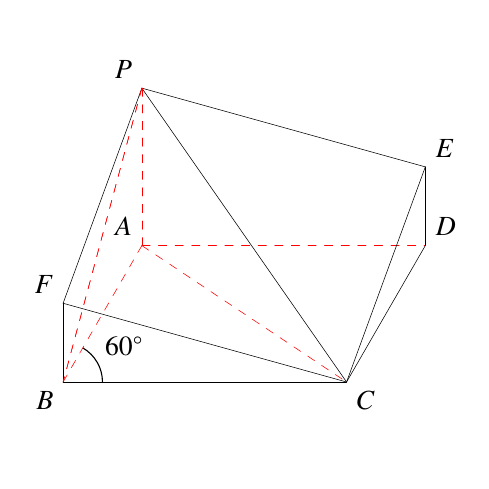
\begin{tikzpicture}[
    scale=1.0,
    decoration={
      markings,
      mark=at position 3cm with {\arrow[scale=2]{>}};
    }]
    % 初始化
    \tkzInit[xmin=-0.25,xmax=5.25, ymin=-1.00,ymax=4.5] \tkzClip    
    % 定义B、C坐标
    \tkzDefPoints{0.2/0/B, 3.8/0/C}
    % 绘制线段BC
    \tkzDrawSegments(B,C)
    % 标记线段B、点符号
    \tkzLabelPoints[below left](B)
    \tkzLabelPoints[below right](C)
    % 利用相对位置,用极坐标定义D点
    \tkzDefShiftPoint[C](60:2){D}
    % 利用相对位置,计算并定义平行四边形最后A
    \tkzDefPointWith[colinear= at D](C,B) \tkzGetPoint{A}
    % 标记线段A、D端点符号
    \tkzLabelPoints[above left](A)
    \tkzLabelPoints[above right](D)
    % 绘制虚线线段AD,BC
    \tkzDrawSegments[color=red, dashed](A,D)
    \tkzDrawSegments[color=red, dashed](B,A)
    % 绘制实线线段CD
    \tkzDrawSegments(C,D)
    % 定义过A点垂直于AD,长度为3.46个单位长度的点P
    \tkzDefPointWith[orthogonal normed,K=2](A,D) \tkzGetPoint{P}
    % 定义过D点垂直于DA,长度为1.73个单位长度的点E
    \tkzDefPointWith[orthogonal normed,K=-1](D,A) \tkzGetPoint{E}
    % 定义过B点垂直于BC,长度为1.73个单位长度的点F
    \tkzDefPointWith[orthogonal normed,K=1](B,C) \tkzGetPoint{F}
    % 标记P、F、E端点符号
    \tkzLabelPoints[above left](P)
    \tkzLabelPoints[above left](F)
    \tkzLabelPoints[above right](E)

    % 绘制实线线段CD
    \tkzDrawSegments(B,F)
    \tkzDrawSegments(D,E)
    \tkzDrawSegments(P,F)
    \tkzDrawSegments(P,E)
    \tkzDrawSegments(P,C)
    \tkzDrawSegments(F,C)
    \tkzDrawSegments(E,C)
    % 绘制实线线段CD
    \tkzDrawSegments[color=red, dashed](P,A)
    \tkzDrawSegments[color=red, dashed](P,B)
    \tkzDrawSegments[color=red, dashed](A,C)
    \tkzDrawSegments[color=red, dashed](P,B)

    % 标记角度
    \tkzMarkAngle[size=0.5](C,B,A)
    \tkzLabelAngle[pos=0.9](C,B,A){$60^\circ$}
 \end{tikzpicture}
\end{figure}    
  
\end{document}

%%% Local Variables:
%%% mode: latex
%%% TeX-master: t
%%% End:
